\section{Circuito de ejemplo}

Durante el desarrollo del curso se va a trabajar sobre un circuito como el de la figura \ref{fig:circuito_ejemplo}.

\begin{figure}[H]
	\centering
	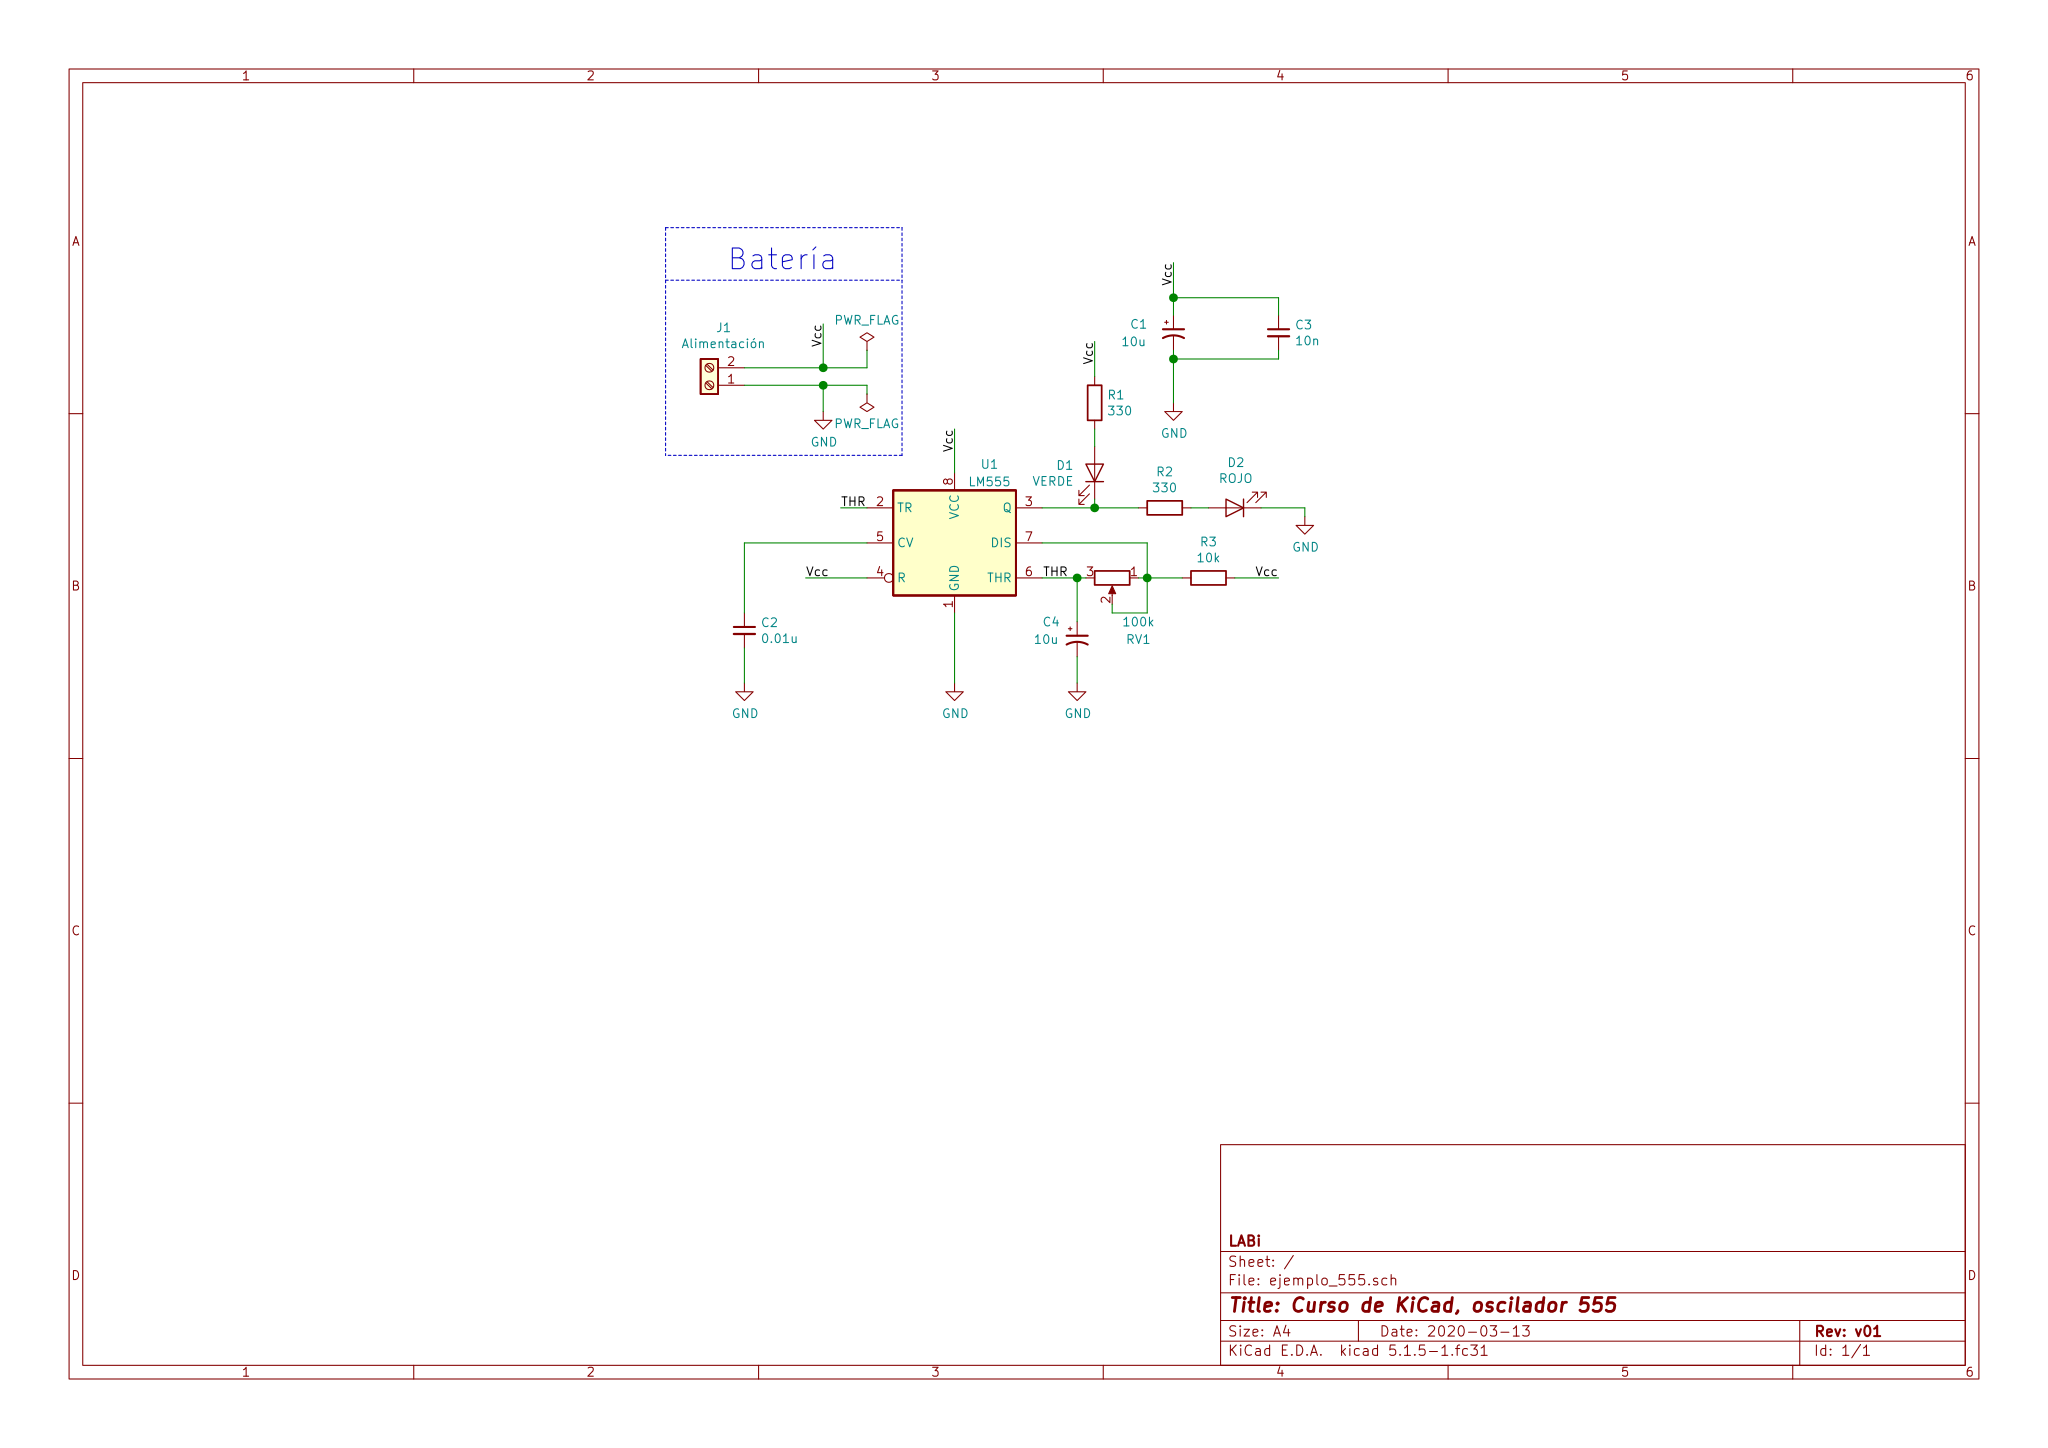
\includegraphics[width=0.5\textwidth]{imagenes/ejemplo_555.png}
	\caption{Circuito oscilador de leds, utilizando el integrado 555.}
	\label{fig:circuito_ejemplo}
\end{figure}

Primero se mostrará cómo armar el esquemático, luego hacer la asociación de huellas y por último diseñar el PCB.